\documentclass[a4paper, twoside]{report}

%% Language and font encodings
\usepackage[english]{babel}
\usepackage[utf8]{inputenc}
\usepackage[T1]{fontenc}
\usepackage{booktabs}
\usepackage{placeins}
\usepackage{tabularx}
\usepackage{longtable}
\setcounter{secnumdepth}{3}
\usepackage{array}
\usepackage{subcaption}
\usepackage[table]{xcolor}
\usepackage{multirow}
\usepackage{verbatim}

\newcolumntype{M}[1]{>{\centering\arraybackslash}m{#1}}

%% Sets page size and margins
\usepackage[a4paper,top=3cm,bottom=2cm,left=3cm,right=3cm,marginparwidth=1.75cm]{geometry}

%% Useful packages
\usepackage{amsmath}
\usepackage{amssymb}
\usepackage{graphicx}
\usepackage[colorinlistoftodos]{todonotes}
\usepackage[colorlinks=true, allcolors=blue]{hyperref}
\usepackage{fancyhdr}

\usepackage{parskip}

%% Diagrams
\usepackage{tikz}
\usetikzlibrary{shapes.geometric, arrows.meta, positioning, calc, fit,
                backgrounds, decorations.pathreplacing, angles, quotes, patterns}

\begin{document}
\begin{titlepage}
\thispagestyle{empty}

\newcommand{\HRule}{\noindent\rule{\textwidth}{0.5mm}}
\newcommand{\ReportTitle}{The LINKU TV2 Experiment: Protocol, Parameters and Record}

%----------------------------------------------------------------------------------------
%	LOGO SECTION
%----------------------------------------------------------------------------------------

\noindent
\begin{minipage}[t]{0.15\textwidth}
    
\includegraphics[width=2cm]{title/Logo_APSCO.png}
\end{minipage}%
\hfill
\begin{minipage}[t]{0.8\textwidth}
    \raggedleft
    {\Huge \textbf{APSCO}}
\end{minipage}
\HRule

%----------------------------------------------------------------------------------------
%	HEADING SECTIONS
%----------------------------------------------------------------------------------------

\begin{center}
\vspace{0.5cm}
{\textbf{\LARGE LINKU Project}\par}
\vspace{0.5cm}
{\textsc{\Large Camera System Working Document}\par}
\vspace{1cm}
\vspace{0.25cm}
{\textsc{\Large "Integrated Instrument, Dark Studio, Tether in Motion"}\par}
\vspace{0.5cm}

%----------------------------------------------------------------------------------------
%	DATE SECTION
%----------------------------------------------------------------------------------------

{\Large \today\par}
\vspace{0.5cm}
\nointerlineskip

%----------------------------------------------------------------------------------------
%   TITLE SECTION
%----------------------------------------------------------------------------------------

\HRule
\vspace{0.20cm}
{\huge \bfseries \ReportTitle\par}
\vspace{0.20cm}
\HRule
\end{center}

%----------------------------------------------------------------------------------------
%	DOCUMENT INFORMATION SECTION
%----------------------------------------------------------------------------------------

\vspace{0.2cm}
\begingroup
\large
\setlength{\parindent}{0pt}
\raggedright

\textbf{Prepared by:}\par
\vspace{0.2cm}

\textsuperscript{1} Pontificia Universidad Catolica del Peru (PUCP)\par
\vspace{0.1cm}


\textbf{Author(s):} Jose Sifuentes\textsuperscript{1}\par
\vspace{0.2cm}

\textbf{Status:} Protocol and acceptance criteria registered, session not yet recorded\par
\vspace{0.5cm}

\textbf{Issue:} 1\par
\textbf{Revision:} 0
\endgroup

%----------------------------------------------------------------------------------------
%	BOTTOM LOGOS
%----------------------------------------------------------------------------------------

\vfill
\begin{center}
    
\includegraphics[width=1\textwidth]{title/Logo_LINKUTEAM.png}
\end{center}

\end{titlepage}


\begin{abstract}
This document is the operating record of the LINKU TV2 experiment: the first
end-to-end run of the camera payload on the integrated support, inside the
blacked-out television studio of the PUCP Faculty of Communications, imaging a
physical tether in motion. It states what the experiment must establish, fixes
every parameter that has to be set before the room is entered, gives the order
in which the session is run, and defines in advance what will count as a pass.

The document exists because three of the project's other deliverables each
defer the same decision to a future self: none of them states a quantitative
threshold against which a result would be judged, and the camera system report
carries no reconstruction accuracy figure at all. Chapter \ref{chap:criteria}
closes that gap for this experiment by registering the criteria \emph{before}
the data exists, which is the only point at which they can be set honestly.

Chapter \ref{chap:objectives} states the objectives and what each one is
evidence for. Chapter \ref{chap:criteria} registers the acceptance criteria.
Chapter \ref{chap:setup} describes the facility and the instrument as built.
Chapter \ref{chap:parameters} collects every parameter to be set and locked,
each with its derivation and its source. Chapter \ref{chap:procedure} gives the
session procedure, whose ordering is load-bearing. Chapter \ref{chap:record}
defines what is written down and how the captures are named, so the session can
be replicated in Blender afterwards. Chapter \ref{chap:analysis} specifies the
analysis to be run on the captures.

\textbf{Status.} Everything that does not depend on results is complete. The
results chapter is empty by construction: at the time of writing no capture
from this experiment exists in the repository, and the record sheet of the
pre-session parameter artifact is blank. Chapter \ref{chap:results} is the
place those go, and it states exactly what must be filled in.
\end{abstract}

\tableofcontents
\listoffigures
\listoftables

\chapter*{Introduction}
\addcontentsline{toc}{chapter}{Introduction}

The LINKU camera payload measures a thin tether strung between two satellites.
It returns metric scalars about that tether, its arc length, straightness,
depth range, diameter and curvature, and a sparse point cloud as a by-product.
Every stage of the processing chain has been built and exercised, and the
optical and photometric requirements have been derived from primary sources in
the companion deliverables. What has not happened is the thing all of it exists
for: the instrument has never been pointed at a real tether, in the dark, on
the support it will actually fly on, with the tether and the rig both in
motion.

That is this experiment. In the project work plan \cite{linku_workplan} it is
the package \emph{Experimento de caja negra, hilo en movimiento}, inside the
phase-2 deliverable \emph{Integracion y experimento en la estructura LINKU}. It
is run in a blacked-out television studio of the PUCP Faculty of
Communications, referred to throughout this document as \textbf{TV2}, a space
borrowed for the purpose because it offers what the project needs and does not
own: a room that can be made genuinely dark, with professional lighting
fixtures and the rigging to position them.

\section*{Why this document exists}

Three reasons, in order of importance.

\textbf{First, the acceptance criteria have to be written down before the data
exists.} This is not a point of style. A review of the project's own
deliverables shows the same gap in three of them independently: the
rolling-shutter experiment and the Blender validation each carry a pending item
instructing a future author to define the quantitative agreement threshold
before running, rather than after seeing the results; the calibration method
leaves three of its four acceptance criteria numerically unset; and the camera
system report \cite{linku_d5_camera_report} contains no reconstruction accuracy
figure at all, reporting its two reconstruction scenarios qualitatively. The
common root is that no mission accuracy budget for tether reconstruction has
been written anywhere in the project. This document cannot supply that budget,
but it can refuse to inherit the habit. Chapter \ref{chap:criteria} registers
the criteria for this experiment in advance.

\textbf{Second, the parameters are scattered and some of them are
destructive to get wrong.} The illumination requirements live in one
deliverable, the optical discipline in another, the calibration preconditions
in a third, and the angular-rate limits in a fourth. On the day, in a borrowed
room, with a time slot, nobody is going to open four documents. Chapter
\ref{chap:parameters} collects all of them in one place, each with its
derivation and its source, and marks which are physics and which are project
decisions open to revision.

\textbf{Third, the session has to be replicable in Blender afterwards.} The
Blender validation deliverable \cite{linku_blender_validation} compares a real
photograph against a render of the same scene, and it currently cannot proceed
because the laboratory-condition light values in its scene are placeholders and
the physical pose of the tether in the chosen reference pair was never written
down. Chapter \ref{chap:record} defines the record so that this experiment does
not repeat that omission.

\section*{What this document is not}

It is not a specification of the illumination; that is derived from primary
sources in the dark-room deliverable \cite{linku_darkroom_illumination} and is
only summarised here. It is not a calibration procedure; that is specified and
implemented in the calibration deliverable \cite{linku_calibration_method} and
is invoked here as a precondition. It is not an analysis of rotation effects
with a known angular rate; that requires a motorised stage and is a separate
experiment \cite{linku_rollingshutter}. In TV2 both the tether and the rig are
moved \emph{by hand}, erratically and without instrumentation of the motion,
which is a deliberate choice discussed in Section \ref{sec:why-by-hand}.

\section*{Status of this revision}

Chapters \ref{chap:objectives} through \ref{chap:analysis} are complete and do
not depend on results. Chapter \ref{chap:results} is empty: at the time of
writing the repository contains no capture from this session, the most recent
non-simulated stereo pairs dating from February 2026, and the record sheet of
the pre-session parameter artifact has not been filled in. Chapter
\ref{chap:results} states precisely what goes in it.

\chapter{Objectives}
\label{chap:objectives}

The experiment has four objectives. They are listed in the order in which a
failure of one invalidates the ones below it, which is also the order in which
the session is run.

\section{O1. Establish a valid calibration on the integrated support}

The stereo geometry that every reconstructed number depends on has to be
measured on the support that will carry the cameras during the experiment, not
on any other mount. The archived calibration is unusable and the project knows
why: measured over 424 archived frames the median board tilt is
4.4\textdegree, only 39\% of frames exceed 5\textdegree, and not one frame in
the entire archive reaches 45\textdegree, which leaves the focal length
mathematically unrecoverable \cite{linku_calibration_method}. The guided tool
built in response refuses to report a session complete until the accepted
views cover four tilt bins.

This objective is a precondition, not a result. If it fails, objectives O2 to
O4 still produce images, but every metric derived from them is scaled by an
unknown factor and no distance in metres can be quoted.

\section{O2. Confirm the illumination reproduces the orbital condition}

One direction of light, no fill, no bounce, a parallel enough beam, and enough
of it. The requirements and their derivation are in the dark-room deliverable
\cite{linku_darkroom_illumination}; the measurement of whether the TV2 fixtures
actually meet them has never been made, because the room has never been
occupied. The enclosure used until now contains one unspecified bulb whose
irradiance, spectrum and beam behaviour have never been measured.

\section{O3. Run the full pipeline end to end on a real moving tether}

Segment, find the endpoints, trace the path in both images, rectify, match,
triangulate, and compute the metric scalars. Every stage has been exercised on
archived or simulated data. None has been exercised on a tether that was
moving, in a dark room, with the rig also moving.

Two specific failure modes are being looked for, both of which the project has
predicted but never observed in hardware:

\begin{itemize}
    \item \textbf{The parametric matching assumption.} Stage 5 pairs the point
    at $i\%$ along the left path with the point at $i\%$ along the right path.
    This holds only if both traced paths start and end at the same physical
    points on the tether and traverse it at the same rate. When an endpoint is
    occluded, or a path leaves the frame, the error is systematic and silent:
    there is no epipolar check to catch it. A hand-moved tether is the first
    situation in which an endpoint can plausibly leave the frame mid-sequence.

    \item \textbf{Rolling-shutter shear.} At the software's current 15 frame/s
    configuration the 3-pixel shear limit corresponds to roughly
    1.05\textdegree/s \cite{linku_rollingshutter}. Hand motion will exceed
    that. The experiment does not measure the rate, so it cannot quantify the
    shear; what it can establish is whether the tracker and the matching
    survive it at all, and at what point they visibly stop doing so.
\end{itemize}

\section{O4. Record the scene well enough to rebuild it in Blender}

The Blender validation deliverable compares a real photograph against a render
of the same scene, and it is currently blocked on two things this session can
supply: measured laboratory-condition light values, which stand in the scene as
placeholders, and the physical pose of the tether, which for the existing
reference pair was never written down
\cite{linku_blender_validation}. Chapter \ref{chap:record} is written to close
both.

\section{What this experiment deliberately does not do}
\label{sec:why-by-hand}

\textbf{It does not measure angular rate.} There is no servo, no motor and no
rotation stage. Both the tether and the camera rig are moved by hand,
erratically. A quantitative rolling-shutter characterisation needs a commanded
or encoded rate, and that is a separate experiment scheduled in a later phase
\cite{linku_rollingshutter}. Running it here with uninstrumented motion would
produce numbers that look quantitative and are not, which is worse than
producing none.

The choice of hand motion is not merely a concession to the absence of a rig.
The deployment it stands in for is itself not a smooth commanded rotation, and
the question this experiment asks is the coarser one that has to be answered
first: does the pipeline survive uncontrolled motion, or does it fail, and
where.

\textbf{It does not attempt a reconstruction accuracy figure against ground
truth.} No independently measured tether geometry is available at the scale
and in the pose used. What can be checked is internal consistency and physical
plausibility, which is what Chapter \ref{chap:criteria} registers.

\textbf{It does not use the flight sensor.} The IMX708 B0308 is the decided
flight sensor but has not been purchased, with procurement expected the
following year. This experiment uses the IMX477 pair that exists. Every
optical figure quoted in this document is therefore computed for the IMX477
with its 1.55~\textmu m pixel and the fitted 8~mm lens, and does not transfer
to the B0308.

\chapter{Acceptance criteria, registered in advance}
\label{chap:criteria}

This chapter is written before the session. Its thresholds are fixed here so
that the result can be judged against a standard that was not chosen with the
result already in view. Where a threshold is derived from physics, the
derivation is given. Where it is a project decision, it is labelled as one and
is open to revision, but only by amending this chapter in a dated revision,
not silently at analysis time.

\section{Why this chapter is not optional}

A low residual on a degenerate set is not evidence of a good calibration; it
is evidence that the ambiguity was absorbed somewhere. The project has already
been caught by exactly this: the best archived session yields a root-mean-square
reprojection error of 1.50~px, which the existing code classified as merely
high rather than catastrophic, while the same fit gives
$f_x = 2651.79 \pm 22.42$~px, a 0.85\% uncertainty, and a distortion
coefficient $k_3 = 3.129 \pm 3.714$ whose standard deviation exceeds its own
value \cite{linku_calibration_method}. A number that looks acceptable while
the parameters behind it are undetermined is the specific failure this chapter
is designed to prevent repeating at the level of the whole experiment.

\section{A1. Calibration}

\begin{table}[htbp]
\centering
\caption[Calibration acceptance criteria]{Acceptance criteria for the
calibration session that precedes the experiment. All are evaluated by the
guided tool at the end of the session, before any experimental capture is
taken.}
\label{tab:crit-calib}
\begin{tabularx}{\textwidth}{@{}l X l@{}}
\toprule
\textbf{Id} & \textbf{Criterion} & \textbf{Threshold} \\
\midrule
A1.1 & Accepted views covering each of the four tilt bins
       (0--10\textdegree, 10--30\textdegree, 30--45\textdegree,
       45--70\textdegree) & $\geq 3$ per bin \\
A1.2 & Relative standard deviation of $f_x$ and of $f_y$ & $\leq 0.3\%$ \\
A1.3 & Standard deviation of each distortion coefficient, relative to the
       magnitude of that coefficient & $< 1$ \\
A1.4 & Offset of the principal point from the image centre, as a fraction of
       image width & $\leq 5\%$ \\
A1.5 & Capture resolution of the calibration frames & $4056 \times 3040$ \\
A1.6 & Cameras not moved, and focus and aperture rings not touched, between
       calibration and the last experimental capture & binary \\
\bottomrule
\end{tabularx}
\end{table}

\textbf{Derivation of A1.2.} The focal length in pixels sets the scale of
every reconstructed distance directly: a relative error $\delta$ in $f_x$
produces a relative error $\delta$ in every depth. At the nominal working
distance of 3.5~m, holding the scale error from this source below 1~cm
requires $\delta \leq 0.29\%$, which rounds to the registered 0.3\%. The
archived best case is 0.85\%, about three times this.

This is the one threshold in the document that may prove unreachable on this
rig. If it is, the correct response is to record the value achieved and state
that the scale error is correspondingly larger, not to relax the number
afterwards. The figure stands as the requirement the measurement has to be
judged against, whether or not it is met.

\textbf{Derivation of A1.3.} A parameter whose standard deviation exceeds its
own magnitude is not determined by the data; the fit is free to set it to zero
without materially changing the residual. This is a binary sanity check, not a
tuned threshold, and the archived fit fails it on $k_3$.

\textbf{Derivation of A1.4.} A principal point far from the image centre is
the signature of the $[t_x, t_y]$ against $[c_x, c_y]$ degeneracy, in which a
board translation and a principal-point shift become indistinguishable. The
active calibration shows $c_x = 694.8$ on a 1920-pixel-wide image where it
should sit near 960, an offset of 265~px or 13.8\% of the width. The 5\%
threshold is a project decision chosen to sit comfortably below the known
failure and comfortably above the few-percent decentring a real lens
assembly can legitimately show.

\textbf{On A1.5.} The relation $f_x = f / p$ means a calibration is tied to
the effective pixel size of the mode it was captured in, and two of the
IMX477 modes crop as well as bin, so the result cannot simply be rescaled
\cite{raspberrypi_camera_docs}. Every archived session used
$1920 \times 1440$, never the full sensor. This criterion exists because the
single most common way to waste the session is to calibrate in one mode and
capture in another.

\section{A2. Illumination}

Each requirement is taken from the dark-room specification
\cite{linku_darkroom_illumination}, where its derivation from primary sources
is given. Reproduced here as pass or fail conditions with the measurement that
decides them.

\begin{table}[htbp]
\centering
\caption[Illumination acceptance criteria]{Illumination acceptance criteria
and the measurement that decides each.}
\label{tab:crit-light}
\begin{tabularx}{\textwidth}{@{}l X l@{}}
\toprule
\textbf{Id} & \textbf{Criterion and how it is measured} & \textbf{Threshold} \\
\midrule
A2.1 & Stray light: with the fixture off, at the longest exposure to be used,
       no scene structure discernible in either camera & nothing visible \\
A2.2 & Single direction: one fixture, or several with parallel axes. No fill,
       no bounce, no ambient & binary \\
A2.3 & Collimation: width of the penumbra cast by a straight edge held 1~m
       from a white card at the tether position & $\leq 35$~mm \\
A2.4 & Uniformity over the working volume, including the depth axis, as
       $(\max-\min)/(\max+\min)$ on a lux grid & $\leq 5\%$ \\
A2.5 & Illuminance at the tether position & $\geq 2320$~lx \\
A2.6 & Short-term stability over the session & $\leq 2\%$ \\
A2.7 & Flicker: white card imaged at the shortest exposure in use, each
       camera & no banding \\
A2.8 & Colour temperature & 5600--6000~K \\
\bottomrule
\end{tabularx}
\end{table}

\textbf{On A2.3.} The real Sun subtends 0.533\textdegree{} and would cast a
9.3~mm penumbra at 1~m \cite{prsa2016iau}. The registered 35~mm corresponds to
a source of about 2\textdegree, set just outside the 1.9\textdegree{} of the
ESA Large Space Simulator \cite{esa_lss}. The virtue of this test is that it
needs a ruler rather than an optical bench.

\textbf{On A2.4.} This is the class B uniformity of IEC 60904-9, using that
standard's own definition \cite{iec60904_9_2020}. The depth axis is the one
that fails first and the one most often omitted from a uniformity check. The
procedure in Chapter \ref{chap:procedure} loops back on failure of this
criterion specifically, because moving a fixture to fix uniformity changes
the illuminance while dimming it does not change the uniformity.

\textbf{On A2.5.} Derived from the Sony IMX477 datasheet
\cite{sony_imx477_datasheet} for the fitted 8~mm f/1.6 configuration at the
1\textdegree/s reference rate, as the illuminance at which a white surface
reaches saturation within the maximum exposure that rate allows. It is a
floor, not a target: four stated assumptions in the derivation all push the
real requirement upward, and a tether darker than a white card needs more.

\textbf{On A2.7.} A mains-connected fixture modulates at twice the line
frequency, giving a 10~ms cycle at 50~Hz, the same order as the exposures in
use, and a rolling shutter turns that into banding
\cite{sheinin2018rollingac}. Note that a global-shutter sensor is not immune:
it converts the banding into frame-to-frame brightness variation, which is
equally destructive for a stereo pair that has to be radiometrically
consistent. Tuning the exposure to an exact multiple of the flicker period is
not available as a remedy, because the exposure is not free. The fixture
itself must not flicker.

\section{A3. Pipeline}

These are evaluated after the session, on the captures, by running the
application unmodified.

\begin{table}[htbp]
\centering
\caption[Pipeline acceptance criteria]{Pipeline acceptance criteria. Unless
stated otherwise each is evaluated on every stereo pair selected for analysis,
and the criterion is met if the stated fraction of pairs passes.}
\label{tab:crit-pipeline}
\begin{tabularx}{\textwidth}{@{}l X l@{}}
\toprule
\textbf{Id} & \textbf{Criterion} & \textbf{Threshold} \\
\midrule
A3.1 & Segmentation yields a tether mask that is a single connected component
       in both images & $\geq 80\%$ of pairs \\
A3.2 & Endpoint detection returns exactly two endpoints in both images &
       $\geq 80\%$ of pairs \\
A3.3 & Automatic tracking reaches the far endpoint without operator
       intervention & $\geq 50\%$ of pairs \\
A3.4 & Fraction of path samples surviving the disparity and depth filters of
       \texttt{compute\_wire\_metrics} & $\geq 90\%$ per pair \\
A3.5 & Reconstructed arc length against the tape-measured tether length, on
       pairs where the whole tether is in frame in both cameras &
       within $\pm 10\%$ \\
A3.6 & Straightness, on a pair where the tether was deliberately held taut &
       $\geq 0.97$ \\
A3.7 & At least one complete run producing an exported point cloud and a full
       set of metric scalars & $\geq 1$ \\
\bottomrule
\end{tabularx}
\end{table}

\textbf{On A3.3.} The 50\% threshold is deliberately lower than the others.
Automatic tracking is the stage most exposed to crossings and to breaks in the
mask, and the application offers a hand-drawn path as a first-class
alternative precisely because the automatic route is not expected to be
universally reliable yet. A result below 50\% is informative rather than
disqualifying: it is the measurement that would justify building the learned
branch scorer.

\textbf{On A3.4.} \texttt{compute\_wire\_metrics} discards points with
non-positive disparity or with $Z$ outside 0.05 to 50~m \emph{before}
computing arc length, so a mid-tether segment that gets filtered makes the
reported total length too short with no warning anywhere in the output. The
retained fraction therefore has to be recorded alongside the length, or the
length cannot be interpreted. This criterion exists to force that.

\textbf{On A3.5.} This is the only criterion in the document that compares
against an external measurement. The tether length is measured with a tape
before the session and recorded in Chapter \ref{chap:record}. The
$\pm 10\%$ tolerance is a project decision and is loose on purpose for a first
run: it has to accommodate the focal scale error permitted by A1.2, the
systematic error of the parametric matching assumption, and the under-reporting
caused by A3.4, none of which has ever been measured together on hardware. It
is set to detect a gross failure, not to certify an accuracy. Tightening it is
the job of the next revision, once there is a measured distribution to tighten
it against.

\textbf{On A3.6.} Straightness is reported by the pipeline as the ratio of
the endpoint chord to the traced arc length, so a taut tether should return a
value just below 1. The 0.97 threshold allows roughly 3\% of path wander from
sag, mask noise and tracking jitter combined.

\section{A4. Record}

\begin{table}[htbp]
\centering
\caption[Record acceptance criteria]{Completeness criteria for the session
record. These decide whether the experiment can be replicated and rendered,
not whether it succeeded.}
\label{tab:crit-record}
\begin{tabularx}{\textwidth}{@{}l X@{}}
\toprule
\textbf{Id} & \textbf{Criterion} \\
\midrule
A4.1 & Every field of the record sheet in Chapter \ref{chap:record} filled, or
       explicitly marked not measured with the reason \\
A4.2 & Tether physical pose recorded: approach angle, distance to the camera
       baseline, and attachment points \\
A4.3 & Fixture make, model, modifier, count and ballast or driver mode
       recorded \\
A4.4 & Ring marks checked and photographed at the end of the session, and the
       result recorded \\
A4.5 & Calibration session and all experimental captures committed to the
       repository, with their per-pair metadata \\
\bottomrule
\end{tabularx}
\end{table}

\textbf{On A4.4.} The experiment moves the rig by hand. Moving the focus ring
changes the focal length, and $f_x$ is the focal length in pixels, so 1\% of
drift is 1\% of scale error on every reconstructed distance. It is a
systematic bias and averaging more frames does not remove it. If the marks
have moved by the end of the session, the data is in doubt and A3.5 cannot be
interpreted; this is the reason the check is a criterion and not a note.

\textbf{On A4.5.} The Blender validation deliverable records that for its
chosen reference pair the capture session and exported point cloud were never
pushed to the repository, leaving only screenshots
\cite{linku_blender_validation}. This criterion exists so that it does not
happen twice.

\section{Overall verdict}

The experiment is reported as a \textbf{pass} if A1, A2 and A4 are met in full
and A3 is met except for A3.3 and A3.5. It is reported as a \textbf{qualified
pass} if A1 and A4 are met, A2 fails on no more than one of A2.3, A2.4 or
A2.8, and A3.7 is met: in that case the captures are usable for geometry but
not as the photometric reference for the Blender comparison. It is reported as
a \textbf{fail} if A1 is not met, because then no quantity in metres means
anything, or if A3.7 is not met, because then the pipeline did not complete
even once.

\chapter{Facility and instrument}
\label{chap:setup}

\section{The venue}

TV2 is a television studio of the PUCP Faculty of Communications, borrowed for
the session through internal services. The project does not own a space that
can be made dark at this scale, and the studio offers three things the
experiment needs and the laboratory enclosure does not: a room that can be
blacked out completely, professional lighting fixtures with the rigging to
position and aim them, and enough floor depth to place a fixture far from the
subject, which is what the collimation requirement A2.3 ultimately demands.

A studio also brings two hazards that the acceptance criteria are written to
catch. Studio lighting is designed for an aesthetic result, so fill light,
bounce and multiple sources are the norm and have to be deliberately
suppressed, which is criterion A2.2. And studio fixtures are frequently
dimmed, often by a method whose modulation frequency is unknown, which is
criterion A2.7.

\section{The instrument, as built}

\begin{table}[htbp]
\centering
\caption[Instrument configuration]{The camera payload as assembled for this
experiment. The integrated support was completed and verified working on 13
October 2026; it is the geometry the calibration must be performed on.}
\label{tab:instrument}
\begin{tabularx}{\textwidth}{@{}l X@{}}
\toprule
\textbf{Item} & \textbf{Configuration} \\
\midrule
Compute & Raspberry Pi Compute Module 5, Cortex-A76 at 2.4~GHz, 16~GB \\
Sensors & Two Arducam HQ 477 modules, Sony IMX477, 12.3~MP
          \cite{sony_imx477_datasheet} \\
Lenses & Arducam C1508ZM04, 8~mm, f/1.6 to f/16, C-mount
         \cite{arducam_c1508zm04} \\
Baseline & 100~mm, fixed by the integrated support \\
Capture & $4056 \times 3040$, 12-bit sensor mode, explicit
          \texttt{-{}-mode} argument \\
Preview & $1920 \times 1440$, used for guidance only, never for measurement \\
Frame rate & 15~frame/s in the current software configuration \\
Synchronisation & Sequential software triggering, with the inter-camera delay
                  recorded per pair \\
Calibration target & ChArUco $5 \times 7$, 37~mm squares, 29.6~mm markers,
                     \texttt{DICT\_6X6\_250} \cite{garrido2014aruco} \\
\bottomrule
\end{tabularx}
\end{table}

\textbf{On the calibration target.} It is a ChArUco pattern printed on paper
and mounted on a rigid folder. Two properties of a target matter and neither
is usually verified: flatness and detectability. Detectability is the reason
for ChArUco rather than a plain chessboard, since a self-identifying target
labels every corner individually and tolerates partial views, which is what
makes interactive guidance possible \cite{rojtberg2018pose}. Flatness has
never been measured for this board, and a paper sheet on a folder is the
weaker of the two properties. It is recorded here as a known limitation
rather than as a controlled parameter.

\textbf{On synchronisation.} Hardware triggering is not exposed through the
standard development configuration, so the two cameras are triggered
sequentially in software. The camera system report asserts this is adequate
for target motion below roughly 5~cm/s \cite{linku_d5_camera_report}; that
bound is an assumption rather than a measured synchronisation error. Hand
motion will exceed it. The inter-camera delay is recorded per pair, and pairs
whose delay is large are candidates for exclusion from A3.5. For reference,
the February 2026 reference pair records a 10.4~ms delay.

\section{The subject}

A physical tether proxy, nominally 1~mm in diameter, strung across the LINKU
structure. The structure itself is built by another member of the team and is
outside the scope of this document; what matters here is that the tether is
attached to it at two points whose positions are recorded, and that the
camera support is mounted on it.

The 1~mm figure is the physical proxy actually used in the laboratory. It
should not be confused with the 0.8~mm figure that appears in the camera
system report, which is explicitly described there as a conservative
assumption adopted for the analytical detectability estimate and is not a
measurement of anything \cite{linku_d5_camera_report}.

\section{Working distance and what the optics do at it}

The nominal working distance is 3.5~m, taken from the Blender replica of the
structure. At that distance, with the fitted 8~mm lens on the IMX477, the
tool \cite{linku_dof_visualizer} gives the figures in Table
\ref{tab:optics-at-work}.

\begin{table}[htbp]
\centering
\caption[Optical behaviour at the working distance]{Optical behaviour of the
fitted configuration at the nominal 3.5~m working distance, computed for the
IMX477 with a 1.55~\textmu m pixel and a one-pixel circle of confusion. These
figures do not transfer to the IMX708 B0308 flight sensor, which has a
different pixel pitch and a different focal length.}
\label{tab:optics-at-work}
\begin{tabularx}{\textwidth}{@{}X l l@{}}
\toprule
\textbf{Quantity} & \textbf{Value} & \textbf{Note} \\
\midrule
Projected width of a 1~mm tether at 3.5~m & 1.47~px & marginally resolved \\
Depth of field focused at 3.5~m, f/1.6 & 3.08 to 4.05~m & 0.96~m total \\
Hyperfocal distance at f/1.6 & 25.8~m & \\
Depth of field focused at 21~m & 11.58 to 112.6~m & tether at 3.5~m is blurred \\
Airy disc diameter at f/1.6 & 2.15~\textmu m & 1.39~px \\
Maximum exposure at the 1\textdegree/s reference rate & 11.1~ms & 1~px blur budget \\
Minimum illuminance to saturate a white card in that exposure & 2320~lx & criterion A2.5 \\
\bottomrule
\end{tabularx}
\end{table}

Two consequences drive the procedure in Chapter \ref{chap:procedure}.

\textbf{The depth of field is under a metre.} Focusing for a far subject does
not merely reduce sharpness at 3.5~m, it moves the near limit of the sharp
zone out to 11.6~m and leaves the tether entirely outside it. The focus has to
be set by looking at a live image at full resolution, at the real distance,
and then locked.

\textbf{The focus ring carries no usable scale.} Its full travel moves the
lens by 0.45~mm, and the last 0.003~mm of that, 0.7\% of the rotation, covers
everything from 21~m to infinity. Setting focus by reading a number off the
barrel is not a viable method on this lens.

\chapter{Parameters to set and lock}
\label{chap:parameters}

Chapter \ref{chap:criteria} says what will be judged. This chapter says what
has to be set, in what order, and why each setting is what it is. The numeric
thresholds are not repeated here; they are in Tables \ref{tab:crit-calib} to
\ref{tab:crit-record}.

Each entry is marked \textbf{Physics} if the Sun or the sensor fixes it and
the project cannot negotiate, or \textbf{Decision} if it is a project choice
that could be revised with an argument.

\section{Illumination}

\subsection*{L1. One direction of light. \textnormal{Physics}}

In orbit the tether is lit by a single distant source and there is no
atmosphere to fill the shadows: the lit side is at full sun and the shadowed
side is nearly black. Several fixtures are permitted only if their axes are
parallel. Converging beams are forbidden, and this is the most important
prohibition in the chapter: two converging sources put two shadows and two
specular highlight lines on a target that is one or two pixels wide, which
presents the matching stage with a doubled thread, a failure mode it is not
designed to handle. Also forbidden are mixing fixture types or colour
temperatures along a row, and placing a fixture at one end shining along the
tether, which combines grazing incidence with inverse-square falloff along
its length.

\subsection*{L2. Daylight colour. \textnormal{Decision}}

Every space vision laboratory in the reviewed set that declares a colour
temperature falls in the daylight range, and the DLR EPOS sun simulator is a
6000~K HMI with CRI 90 \cite{dlr2025eposportfolio, benninghoff2017epos}. The
Sun's effective temperature is 5772~K \cite{prsa2016iau}. This rules out
3200~K tungsten without further discussion. TLCI is requested as a datum
because CRI was not designed for cameras \cite{ebu_tech3355}, but no TLCI
threshold is set, because no reviewed source gives one.

\subsection*{L3. Parallel beam. \textnormal{Decision, anchored to physics}}

Verified with the penumbra test of Section \ref{sec:penumbra}. There is a
second, independent reason for collimation beyond matching the Sun's shadow
behaviour: without it, the inverse-square falloff makes the uniformity
requirement L4 unachievable at any distance that fits in the room. A point
source would need a throw of roughly twenty times the object depth to reach
class B uniformity, which is about 10~m for a 0.5~m deep structure and 20~m
for a 1~m one. Few rooms offer that.

\subsection*{L4. Uniformity across the working volume, depth included.
\textnormal{Decision, from IEC class B}}

Measured on a lux grid that spans width, height and depth. The depth axis
fails first and is the one most often left out.

\subsection*{L5. Enough light at the tether. \textnormal{Physics, from the
datasheet}}

Derived in the dark-room deliverable from the IMX477 datasheet. It is a
floor. Four assumptions enter the derivation, all of which push the true
requirement upward: the datasheet's 3200~K test spectrum differs from the
5600 to 6000~K in use; the treatment of sensor gain; an on-axis transmittance
of unity, ignoring vignetting; and a white card of reflectance 0.9 filling
many pixels, where the real tether is darker and narrower.

\subsection*{L6. No flicker. \textnormal{Physics}}

For an HMI, use an electronic ballast in its high-frequency mode, near
1000~Hz. Note specifically that the ARRI EB 12/18 manual states its
``50/60~Hz, low noise'' mode is \emph{not} flicker free despite the ballast
being an electronic one, and that its 75~Hz ``flicker free'' mode is also
unsuitable here because the resulting period exceeds the exposure ceiling set
by the rotation rate \cite{arri_eb1218_manual}. Magnetic ballasts are
excluded. For an LED fixture, request the dimming method and the PWM
frequency from the supplier; no reviewed source gives a safe value, so the
fixture is accepted only after the on-site test A2.7.

\subsection*{L7. Black surroundings, fixture out of frame.
\textnormal{Decision}}

Black velvet or molton, no light falling on walls. This is how DLR and
Stanford build their testbeds \cite{benninghoff2017epos, park2021tron}, and
black velvet was the best background measured with the same Raspberry Pi HQ
camera this project uses \cite{pauly2022spacelab}. A fixture inside the frame
produces flare; Stanford report exactly that when the camera points near their
sun lamp. IEC 60904-9 separately warns that wall reflections invalidate a
measured uniformity classification \cite{iec60904_9_2020}.

\section{The penumbra test}
\label{sec:penumbra}

Hold a straight edge 1~m in front of a white card placed at the tether
position, and measure the width of the diffuse band with a ruler. The geometry
is
\begin{equation}
w = L \tan \alpha ,
\label{eq:penumbra}
\end{equation}
where $L$ is the edge-to-card distance and $\alpha$ the angular size of the
source as seen from the edge. The measured width therefore gives the angular
size directly. The Sun would give 9.3~mm at $L = 1$~m; the registered limit of
35~mm corresponds to about 2\textdegree; an uncollimated lamp typically gives
87~mm or more. The value of this test is that it converts an optical property
into a ruler reading.

\section{Optics}

\subsection*{O1. Aperture wide open at f/1.6. \textnormal{Decision, with
calculation}}

Two independent arguments point the same way. Stopping down costs light as
the square of the f-number: going to f/2.8 triples the illuminance
requirement, from 2320 to about 7100~lx. And diffraction is already
significant wide open, with the Airy disc at 2.15~\textmu m or 1.39~px at
f/1.6, rising to 2.42~px at f/2.8 and 4.85~px at f/5.6, against a tether that
projects to 1.47~px. There is no aperture at which closing down helps.

\subsection*{O2. Focus at the real tether distance, set by eye.
\textnormal{Physics}}

Set while looking at the live image at full resolution, with the tether in
place. See Chapter \ref{chap:setup} for why the barrel scale cannot be used.

\subsection*{O3. Lock and mark both rings. \textnormal{Critical}}

Tighten the grub screws and mark the ring positions with a pen or tape.
Moving focus changes the focal length, and $f_x$ is the focal length in
pixels, so 1\% of drift is 1\% of scale error on every reconstructed distance,
or 10~mm per metre. It is a systematic bias and averaging does not remove it.
This experiment moves the rig by hand, so a loose ring will move. The marks
are checked at the end of the session, which is criterion A4.4.

\section{Calibration}

\subsection*{C1. Same resolution and same sensor mode as the experiment.
\textnormal{Physics}}

Capture the calibration frames at $4056 \times 3040$ with an explicit
\texttt{-{}-mode}. Without that argument libcamera may silently pick a mode
and then scale or crop, which makes the transfer untrustworthy
\cite{raspberrypi_camera_docs}.

\subsection*{C2. Calibrate on the integrated support. \textnormal{Physics}}

The stereo extrinsics describe the rigid transform between two specific
cameras in specific positions. Calibrating on one mount and then moving the
cameras to another invalidates them. The support is already built; the
calibration session happens on it, in the room, with the structure in place.

\subsection*{C3. Fill all four tilt bins. \textnormal{Physics}}

This is the correction for the diagnosed cause of the 23 previous failures.
With the board nearly parallel to the sensor in every view, a longer focal
length at a greater distance produces an identical image and the focal length
is simply not recoverable, however many frames are taken
\cite{zhang2000flexible, linku_calibration_method}. The guided tool asks for a
specific pose, draws its outline in both previews, and only accepts a frame
that is on that pose, so filling the bins is the tool's job rather than the
operator's; what the operator has to do is physically reach the poses it asks
for, including the strongly tilted ones.

\subsection*{C4. Do not touch the optics afterwards. \textnormal{Critical}}

See O3. Calibration and experiment are one continuous optical configuration.

\section{Camera settings during the checks and the run}

Base gain, fixed white balance, manual exposure at the ceiling given in Table
\ref{tab:optics-at-work}. Automatic exposure and automatic white balance are
both disabled: an auto-exposure loop will chase the moving tether and change
the radiometry from frame to frame, which breaks both the flicker test and the
stereo consistency the matching depends on.

\chapter{Session procedure}
\label{chap:procedure}

\section{Why the order matters}

The sequence below is not a checklist that can be reordered for convenience.
The geometric settings are fixed before the photometric ones for a specific
reason: \textbf{moving a fixture to correct uniformity changes the
illuminance, while dimming it does not change the uniformity}. Settle
position and aim first, then level. Doing it the other way round means
measuring the light twice.

The same logic places calibration after the optics are locked and before any
experimental capture, and places the stray-light check before everything,
because a room that is not actually dark invalidates every photometric number
measured in it.

\begin{figure}[htbp]
\centering
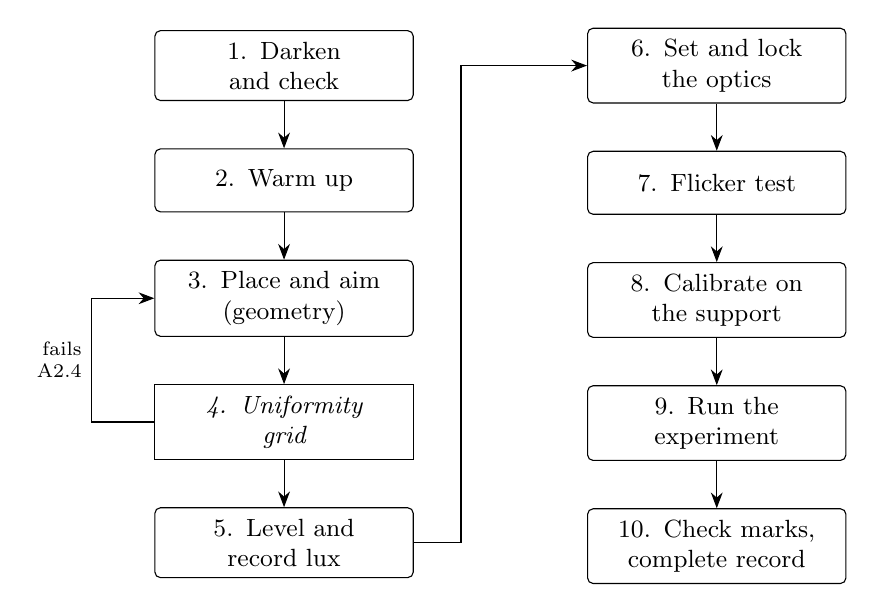
\begin{tikzpicture}[
  node distance = 6mm and 10mm,
  box/.style  = {draw, rounded corners=2pt, align=center, inner sep=4pt,
                 font=\small, minimum height=8mm, text width=30mm},
  gate/.style = {draw, align=center, inner sep=4pt, font=\small\itshape,
                 minimum height=8mm, text width=30mm},
  ar/.style   = {-{Stealth[length=2mm]}}
]
\node[box] (s1) {1. Darken \\ and check};
\node[box, below=of s1] (s2) {2. Warm up};
\node[box, below=of s2] (s3) {3. Place and aim \\ (geometry)};
\node[gate, below=of s3] (s4) {4. Uniformity \\ grid};
\node[box, below=of s4] (s5) {5. Level and \\ record lux};
\node[box, right=22mm of s1] (s6) {6. Set and lock \\ the optics};
\node[box, below=of s6] (s7) {7. Flicker test};
\node[box, below=of s7] (s8) {8. Calibrate on \\ the support};
\node[box, below=of s8] (s9) {9. Run the \\ experiment};
\node[box, below=of s9] (s10) {10. Check marks, \\ complete record};

\draw[ar] (s1) -- (s2);
\draw[ar] (s2) -- (s3);
\draw[ar] (s3) -- (s4);
\draw[ar] (s4) -- (s5);
\draw[ar] (s5.east) -- ++(6mm,0) |- (s6.west);
\draw[ar] (s6) -- (s7);
\draw[ar] (s7) -- (s8);
\draw[ar] (s8) -- (s9);
\draw[ar] (s9) -- (s10);

\draw[ar] (s4.west) -- ++(-8mm,0) |- node[pos=0.25, left, font=\scriptsize,
          align=right] {fails \\ A2.4} (s3.west);
\end{tikzpicture}
\caption[Session procedure]{The session procedure. The only loop is the
uniformity check returning to fixture placement, because correcting
uniformity means moving a fixture, which changes the illuminance and
invalidates any level already measured.}
\label{fig:procedure}
\end{figure}

\section{The ten steps}

\begin{enumerate}
    \item \textbf{Darken the room.} Close, cover, and rig the black
    background. Verify with a frame from each camera at the longest exposure
    that will be used, with the fixture off. Nothing recognisable may appear.
    Anything visible is stray light and must be eliminated before continuing.
    This is criterion A2.1.

    \item \textbf{Warm up the fixture} for the manufacturer's stated time
    before measuring anything. For HMI this is several minutes. If a
    spectroradiometer is used, EBU recommends at least 30 minutes for the
    instrument itself \cite{ebu_tech3355}.

    \item \textbf{Place and aim.} Position the fixture at the greatest throw
    the room allows and set its aim. Run the penumbra test of Section
    \ref{sec:penumbra} and record the width. This is criterion A2.3.

    \item \textbf{Map the uniformity.} Take a lux grid across width, height
    and depth of the working volume. If criterion A2.4 fails, move the
    fixture and return to step 3. Do not attempt to fix uniformity by
    dimming.

    \item \textbf{Record the level.} Illuminance at the tether position,
    against criterion A2.5. Also record the grid minimum and maximum from
    step 4 and the measured colour temperature.

    \item \textbf{Set and lock the optics.} Aperture wide open, focus set by
    eye on the live full-resolution image with the tether in place, then both
    rings tightened and marked. Photograph the marks.

    \item \textbf{Flicker test.} White card, shortest exposure in use, one
    frame from each camera. Look for banding. This is criterion A2.7. If it
    fails, the fixture or its ballast mode has to change, and steps 3 to 5
    are repeated for the replacement.

    \item \textbf{Calibrate} on the integrated support, in place, following
    Section \ref{sec:calib-run}.

    \item \textbf{Run the experiment} following Section \ref{sec:capture-plan},
    touching nothing on the optics.

    \item \textbf{Close out.} Check the ring marks against the photographs
    from step 6 and record whether they moved. Complete every field of the
    record sheet. Copy the captures off the device.
\end{enumerate}

\section{Running the calibration}
\label{sec:calib-run}

The application's guided flow does the bookkeeping. The operator's job is
physical.

The tool asks for one pose at a time and draws its outline in both camera
previews. A frame is captured only when it is sharp over the board region,
momentarily still, visible to \emph{both} cameras, and on the pose currently
being asked for. A rejected frame does not consume a slot, so a request for
25 views yields 25 that passed every gate.

Three practical points for the operator:

\begin{itemize}
    \item \textbf{Stand back and hold the board yourself.} The flow is built
    for a single person holding the board at a distance and matching the
    drawn outline. The preview is sized so it remains readable from across
    the room.

    \item \textbf{The strongly tilted poses are the point.} The bins at 30 to
    45\textdegree{} and 45 to 70\textdegree{} are the ones no archived session
    ever reached, and they are the ones that make the focal length
    recoverable. If a pose cannot be physically reached, use \emph{Finish with
    the views collected}; that is the deliberate way out, and the session
    reports itself as incomplete rather than pretending otherwise.

    \item \textbf{Watch the uncertainty, not the residual.} The progress
    indicator is driven by parameter uncertainty from the fit covariance, not
    by a frame count and not by the reprojection error. A session is finished
    when the uncertainty stops falling, not when a number of frames has been
    reached.
\end{itemize}

At the end, evaluate Table \ref{tab:crit-calib}. If A1 fails, the experiment
can still be run, but Chapter \ref{chap:analysis} will report lengths in
pixels and ratios rather than in metres, and criterion A3.5 is void.

\section{The capture plan}
\label{sec:capture-plan}

Both the tether and the rig are moved by hand. The plan is organised so that
the simplest configurations are captured first, while everything is known to
be working, and the hardest last.

\begin{table}[htbp]
\centering
\caption[Capture plan]{Capture sequence. Each configuration is captured as
several stereo pairs, so that a failure in any one pair does not cost the
configuration. Counts are a minimum.}
\label{tab:capture-plan}
\begin{tabularx}{\textwidth}{@{}l X l@{}}
\toprule
\textbf{Set} & \textbf{Configuration} & \textbf{Pairs} \\
\midrule
S1 & Tether taut and static, whole length in frame in both cameras. The
     reference set for A3.5 and A3.6 & $\geq 5$ \\
S2 & Tether with deliberate sag, static & $\geq 3$ \\
S3 & Tether static, camera rig moved slowly by hand & $\geq 5$ \\
S4 & Tether static, camera rig moved erratically & $\geq 5$ \\
S5 & Tether in motion, rig static & $\geq 5$ \\
S6 & Both in motion, erratic. The nominal case & $\geq 10$ \\
S7 & Tether arranged with a deliberate self-crossing, static & $\geq 3$ \\
S8 & One endpoint deliberately out of frame in one camera only &
     $\geq 3$ \\
\bottomrule
\end{tabularx}
\end{table}

\textbf{S1 is the measurement set.} It is the only one where an external
reference exists, because the tether is taut and its length has been
tape-measured. Everything else is an exercise of robustness.

\textbf{S7 exists to characterise the tracker, not to pass.} A self-crossing
is where the automatic tracker has to choose a branch using a hand-tuned
scoring formula, and it is the case the project expects to be weakest.
Capturing it deliberately turns an anticipated weakness into a measurement,
and the pairs feed the path dataset whether the tracker succeeds or not.

\textbf{S8 exists to provoke a silent failure.} The parametric matching
assumption breaks when the two traced paths do not cover the same physical
extent, and nothing in the pipeline detects it. Deliberately occluding one
endpoint in one camera creates that condition on purpose, so that the size
and the sign of the resulting error can be seen for the first time against
the tape-measured length from S1.

\chapter{What gets recorded}
\label{chap:record}

The session produces two things: image files, which the software names and
stores by itself, and written observations, which nothing records unless a
person writes them down. This chapter specifies the second, because it is the
part that has previously gone missing.

\section{The record sheet}

Every field is filled during the session, not reconstructed afterwards. A
field that could not be measured is marked \emph{not measured} with the
reason, which is criterion A4.1. An empty cell is indistinguishable from a
forgotten one.

\begin{longtable}{@{}p{0.52\textwidth} p{0.13\textwidth} p{0.27\textwidth}@{}}
\caption[Session record sheet]{The session record sheet. Transcribed into the
results chapter after the session.}
\label{tab:record} \\
\toprule
\textbf{Datum} & \textbf{Unit} & \textbf{Value} \\
\midrule
\endfirsthead
\toprule
\textbf{Datum} & \textbf{Unit} & \textbf{Value} \\
\midrule
\endhead
\multicolumn{3}{@{}l}{\textit{Venue and date}} \\
Room, date, start and end time & & \\
People present and their roles & & \\
\addlinespace
\multicolumn{3}{@{}l}{\textit{Fixture}} \\
Make, model, modifier, count & text & \\
Ballast or driver, and the mode selected & text & \\
Dimming method and PWM frequency, if LED & text, Hz & \\
Warm-up time allowed before measuring & min & \\
Distance and angle of the fixture to the structure and to the cameras & m, \textdegree & \\
\addlinespace
\multicolumn{3}{@{}l}{\textit{Photometry}} \\
Illuminance at the tether position & lx & \\
Uniformity grid: minimum and maximum, and the grid spacing used & lx, m & \\
Measured colour temperature & K & \\
Measured CRI, and TLCI if available & & \\
Penumbra width at 1~m & mm & \\
Stability over the session: minimum and maximum & lx & \\
Stray-light check result & pass/fail & \\
Flicker test result, per camera & pass/fail & \\
\addlinespace
\multicolumn{3}{@{}l}{\textit{Geometry of the scene}} \\
Tether physical length, tape measured & m & \\
Tether diameter, measured & mm & \\
Tether material and surface finish & text & \\
Attachment points on the structure, described or sketched & & \\
Tether approach angle relative to the camera baseline & \textdegree & \\
Distance from the camera baseline to the nearest and farthest tether point & m & \\
Working volume of the structure: width, height, depth & m & \\
\addlinespace
\multicolumn{3}{@{}l}{\textit{Optics and cameras}} \\
Focus distance set, and how it was judged & m, text & \\
Aperture set & f/ & \\
Both rings locked and marked, before the session & yes/no & \\
Both marks unmoved, after the session & yes/no & \\
Per camera: exposure, gain, white balance & ms, dB & \\
Capture resolution and sensor mode used & px & \\
\addlinespace
\multicolumn{3}{@{}l}{\textit{Calibration}} \\
Session directory name & text & \\
Accepted views per tilt bin & count $\times$ 4 & \\
Relative standard deviation of $f_x$, $f_y$ & \% & \\
Principal point offset from centre & px, \% & \\
Reported reprojection RMS, for the record only & px & \\
Session reported complete by the tool & yes/no & \\
\addlinespace
\multicolumn{3}{@{}l}{\textit{Captures}} \\
Capture sets obtained, against Table \ref{tab:capture-plan} & S1--S8 & \\
Total stereo pairs & count & \\
Inter-camera delay: median and worst & ms & \\
Anything that went wrong, in prose & & \\
\bottomrule
\end{longtable}

\section{Why the scene geometry fields are there}

The block headed \emph{Geometry of the scene} is not documentation for its
own sake. The Blender validation deliverable selected a real stereo pair as
its reference and then found it could not reproduce the scene, because the
tether's approach angle, distance and attachment points had never been
written down \cite{linku_blender_validation}. Those four fields exist so that
this session's captures do not become unusable for the same reason.

The photometry block serves the same deliverable from the other side: its
laboratory-condition light is currently a placeholder, and these measurements
are what replaces it.

\section{Files, naming and metadata}

The application writes each stereo pair to its own timestamped directory
under \texttt{data/\allowbreak captures/}, with per-pair metadata including the capture
resolution, the baseline and the inter-camera delay. That naming is
automatic and should not be changed by hand. What has to be added is the
mapping from directory to capture set.

\begin{itemize}
    \item Keep a plain text file in the session folder mapping each capture
    directory to its set S1 to S8 and to a one-line description of what was
    being done at the time. Written during the session, not after.

    \item Commit the calibration session directory and every capture
    directory, with their metadata, which is criterion A4.5. The repository
    already versions \texttt{data/\allowbreak captures/} and
    \texttt{data/\allowbreak calibration/}, so this is the default behaviour rather than
    an exception, but it has to actually be done.

    \item Photograph the physical setup: the fixture position, the structure
    with the tether strung, the camera support in place, and the ring marks.
    These go in \texttt{Images/} of this deliverable.
\end{itemize}

\section{What is deliberately not recorded}

The angular velocity of the hand motion. There is no instrumentation for it,
and writing down an estimate would create a number that later analysis would
be tempted to treat as a measurement. Section \ref{sec:why-by-hand} gives the
reasoning. The rolling-shutter deliverable is where that quantity gets
measured, with a stage that either commands or encodes the rate
\cite{linku_rollingshutter}.

\chapter{Analysis plan}
\label{chap:analysis}

The analysis is run after the session, on the committed captures, using the
application without modification. Running a modified pipeline on the
experimental data would mean the result does not describe the software that
exists.

\section{The pipeline, stage by stage}

The measurement path is the \emph{Geometric (Wire Tracking)} mode, which is
the application default. The alternative dense stereo mode is not used, and
Section \ref{sec:no-dense} explains why that matters more than it sounds.

\begin{enumerate}
    \item \textbf{Segmentation.} The cable detection tuner produces a binary
    mask for each image. Two segmenters are available: the classical one,
    based on a top-hat transform with adjustable parameters, and a trained
    random forest operating per pixel on nine hand-crafted features. Record
    which was used for each pair.

    \item \textbf{Endpoint detection.} The mask is skeletonised and pruned,
    and the two endpoints are taken as the geodesically farthest pair.

    \item \textbf{Path tracing.} Either automatic, a depth-first search over
    the mask with backtracking and momentum, or hand drawn by the operator
    clicking along the tether. Record which, per pair: this is what criterion
    A3.3 counts.

    \item \textbf{Rectification} of both images from the calibration.

    \item \textbf{Matching.} The point at $i\%$ along the left path is paired
    with the point at $i\%$ along the right path.

    \item \textbf{Triangulation} into a sparse point cloud, written out
    directly from the disparity and the baseline rather than through
    OpenCV's triangulation routines.

    \item \textbf{Metrics.} Arc length, straightness, depth range, diameter
    and curvature.

    \item \textbf{Export} to PLY, XYZ, PCD or OBJ.
\end{enumerate}

\section{What is computed, and against what}

\begin{table}[htbp]
\centering
\caption[Analysis outputs]{What is extracted from each analysed pair and what
it is compared against.}
\label{tab:analysis}
\begin{tabularx}{\textwidth}{@{}l X X@{}}
\toprule
\textbf{Quantity} & \textbf{Source} & \textbf{Compared against} \\
\midrule
Mask connectivity & stage 1 & criterion A3.1 \\
Endpoint count & stage 2 & criterion A3.2 \\
Tracking mode used, and coverage reached & stage 3 & criterion A3.3 \\
Retained sample fraction & stage 7 & criterion A3.4 \\
Arc length in metres & stage 7 & tape measure, criterion A3.5 \\
Straightness & stage 7 & criterion A3.6, on taut pairs only \\
Depth range & stage 7 & scene geometry record \\
Reported diameter & stage 7 & measured tether diameter \\
Curvature & stage 7 & qualitative, sag pairs \\
\bottomrule
\end{tabularx}
\end{table}

\section{The retained fraction has to be reported with every length}

\texttt{compute\_wire\_metrics} discards samples whose disparity is
non-positive or whose depth falls outside 0.05 to 50~m, and it does this
\emph{before} summing the chord lengths. A tether segment that gets filtered
out therefore shortens the reported arc length, and nothing in the output
says so. A length quoted without its retained fraction is not interpretable,
so the two are always reported together. Criterion A3.4 sets the floor at
90\%.

\section{The comparison that is expected to fail, and why that is useful}

Capture set S8 deliberately places one endpoint outside the frame of one
camera. The matching stage assumes both traced paths span the same physical
extent of the tether, and there is no epipolar check anywhere in the pipeline
that could detect a violation. The predicted consequence is a systematic
error in the reconstructed length with no accompanying warning.

The analysis of S8 is therefore: take the arc length reported for the S8
pairs, compare it against the tape-measured length and against the S1 pairs
of the same tether, and record the magnitude and the sign of the discrepancy.
This is the first time the project would have a measured size for an error it
has only ever reasoned about.

A secondary analysis, if the S8 result is large, is to run the same pairs
through the epipolar matcher that exists in the codebase but is not reachable
from the interface. That matcher does not rely on the parametric assumption
and was kept specifically against this possibility. It has never been
validated on real data, so a result from it is exploratory, not a
measurement.

\section{Why dense stereo is not used, and the trap that creates}
\label{sec:no-dense}

Dense stereo fails on a thin, textureless object because there is nothing
along the wire to correlate. This has already been demonstrated twice:
commercial structure-from-motion on the isolated tether returns a zero
resolution error and produces no camera alignment or sparse cloud at all, the
stated reason being insufficient visual information within the tether itself
rather than background interference; and dense stereo inside the laboratory
enclosure gives correct disparity on a solid target while also producing
non-physical disparity throughout regions that should be empty background,
yielding phantom geometry that needs manual intervention to clean
\cite{linku_d5_camera_report}.

The trap is operational. If the operator does not configure a mask in the
segmentation tuner, the processing falls back to dense stereo
\emph{automatically and silently}. It does not raise an error. It produces
something that looks like a point cloud. Any analysis run after skipping the
tuner is therefore running the method already known to fail, in a form that
looks plausible. The analysis log records, for every pair, that a mask was
present.

\section{Feeding the datasets}

Every pair that is successfully traced, automatically or by hand, is saved
into the path dataset together with its mask and its verified path. This
dataset currently holds three stereo samples against a recommended 30 to 100,
and it is the input to the one model in the plan that does not yet exist: a
learned per-branch scorer that would replace the fixed hand-tuned weights in
the tracker's decision at each crossing.

One caution applies to the other dataset. Saving a sample to the mask dataset
while the random-forest segmenter is active means training the model on its
own unverified output, which reinforces its errors. The application asks for
confirmation in that case; the answer during this session is no, unless the
mask has been inspected and corrected.

\chapter{Results}
\label{chap:results}

\textbf{This chapter is empty. No result exists yet.}

At the time of this revision the repository contains no capture from the TV2
session. The most recent non-simulated stereo pairs in
\texttt{data/captures/} date from February 2026, and the most recent
simulated ones from September 2026. The record sheet of the pre-session
parameter artifact has not been filled in.

Nothing in this chapter should be written before the session. What follows is
the structure to fill, so that the writing afterwards is transcription rather
than reconstruction.

\section{Session record}

Transcribe Table \ref{tab:record} here, completed. Every \emph{not measured}
entry keeps its reason.

\section{Calibration outcome}

Report against Table \ref{tab:crit-calib}: the accepted view count per tilt
bin, the relative standard deviations of $f_x$ and $f_y$, the standard
deviation of each distortion coefficient against its own magnitude, the
principal point offset, and whether the tool reported the session complete.

Report the reprojection RMS as well, but report it \emph{after} the
uncertainties and label it as the training residual it is. If A1.2 was not
met, state the value achieved and carry the implied scale error forward into
every length quoted in this chapter.

\section{Illumination outcome}

Report against Table \ref{tab:crit-light}, one row per criterion, with the
measured value and pass or fail. Where a criterion failed, state what was
tried.

\section{Pipeline outcome}

Report against Table \ref{tab:crit-pipeline}, aggregated across the analysed
pairs, with the per-set breakdown from Table \ref{tab:capture-plan}. Every
arc length is reported with its retained sample fraction beside it.

\section{The two anticipated failure modes}

\textbf{Parametric matching, from set S8.} The measured discrepancy against
the tape-measured length, with its sign, and how it compares to the S1 pairs
of the same tether.

\textbf{Rolling-shutter shear, from sets S4 and S6.} A qualitative
description of whether shear was visible at all, and at what point in the
motion the tracker or the matching visibly stopped working. No angular rate
is quoted, because none was measured.

\section{Verdict}

State the overall verdict using the definitions at the end of Chapter
\ref{chap:criteria}: pass, qualified pass, or fail. State it before
discussing what it means.

\section{What the next session should change}

Written last, from what actually went wrong rather than from what was
anticipated here.

\todo[inline]{Pending: run the session and complete this chapter. Until it is
complete, this deliverable is a protocol, not a report, and should not be
cited as evidence that the instrument has been validated.}

\chapter*{Status and limitations}
\addcontentsline{toc}{chapter}{Status and limitations}

\section*{Where each part stands}

\begin{table}[htbp]
\centering
\caption[Status of this document]{What is settled and what is not.}
\label{tab:status}
\begin{tabularx}{\textwidth}{@{}l l X@{}}
\toprule
\textbf{Part} & \textbf{Status} & \textbf{Basis} \\
\midrule
Objectives & Settled & Derived from the work plan package and from the gaps
             the companion deliverables leave open \\
Acceptance criteria & Registered & Fixed before any data exists. A1.2, A2.x
             and A3.4 derived; A1.4, A3.3, A3.5 and A3.6 are project
             decisions \\
Instrument description & Measured & The hardware exists and was verified
             working on 13 October 2026 \\
Optical figures & Derived & Thin-lens model for the IMX477 with the fitted
             8~mm lens; reproduced independently from first principles \\
Illumination requirements & Derived & From primary sources in the companion
             dark-room deliverable \\
Procedure & Settled & Ordering follows from the physics, not from
             convenience \\
Record sheet & Settled & Scope set by what the Blender comparison needs \\
Analysis plan & Settled & Runs the existing application unmodified \\
Results & \textbf{Absent} & The session has not been recorded \\
\bottomrule
\end{tabularx}
\end{table}

\section*{Limitations that are known before the session}

\textbf{No angular rate is measured.} Both the tether and the rig are moved
by hand. Nothing in this experiment can produce a quantitative
rolling-shutter result, and the document is written so that nothing in it
can be mistaken for one.

\textbf{No independent ground truth except length.} The only external
measurement available is a tape-measured tether length, which constrains
scale but says nothing about shape. Straightness and curvature are judged for
internal consistency and plausibility only.

\textbf{Board flatness is unverified.} The calibration target is paper on a
folder. Flatness is one of the two target properties that matter and it has
never been measured for this board.

\textbf{The sensor is not the flight sensor.} Every optical number here is
computed for the IMX477 with its 1.55~\textmu m pixel and the 8~mm lens. The
decided flight sensor is the IMX708 B0308, which has a different pixel pitch
and a different focal length, and which has not been purchased. None of these
figures transfers to it without recomputation.

\textbf{Synchronisation is sequential and software-timed.} The adequacy bound
of roughly 5~cm/s quoted in the camera system report is an assumption, not a
measured synchronisation error, and hand motion exceeds it.

\section*{What this experiment unblocks}

If it passes, three things that are currently waiting can proceed. The
Blender validation gets measured laboratory light values and a recorded
tether pose, which are its two missing inputs. The path dataset gains the
first real samples of crossings and of partial occlusion, which is the input
to the learned branch scorer. And the project gains, for the first time, a
reconstruction length with a stated uncertainty that can be compared against
something measured with a tape.

If it fails, the most likely place is A1, the calibration, which is the
project's longest-standing open problem and the one with the least margin in
the schedule.

\appendix

\chapter{Constants and their provenance}
\label{app:constants}

Every number used in this document, with where it came from. The status
column distinguishes a measurement from a calculation from an assumption,
because the three carry different weight and the distinction is lost once
they share a table in a slide.

\begin{longtable}{@{}p{0.38\textwidth} p{0.17\textwidth} p{0.38\textwidth}@{}}
\caption[Constants used]{Constants and derived quantities used in this
document.}
\label{tab:constants} \\
\toprule
\textbf{Quantity} & \textbf{Value} & \textbf{Status and source} \\
\midrule
\endfirsthead
\toprule
\textbf{Quantity} & \textbf{Value} & \textbf{Status and source} \\
\midrule
\endhead
\multicolumn{3}{@{}l}{\textit{The Sun}} \\
Total solar irradiance, AM0 & 1361~W/m\textsuperscript{2} & IAU 2015 nominal
  \cite{prsa2016iau} \\
Solar illuminance in orbit & 132\,800~lx & Calculated, AM0 spectrum against
  $V(\lambda)$ \cite{astm_e490_data, cie_vlambda} \\
Solar effective temperature & 5772~K & IAU 2015 nominal \cite{prsa2016iau} \\
Solar angular diameter & 0.533\textdegree & IAU radius and distance
  \cite{prsa2016iau} \\
Penumbra cast by the Sun & 9.3~mm per m & Calculated from the above,
  Eq. \ref{eq:penumbra} \\
\addlinespace
\multicolumn{3}{@{}l}{\textit{Sensor and lens, as fitted}} \\
Sensor & Sony IMX477 & Hardware \cite{sony_imx477_datasheet} \\
Pixel pitch & 1.55~\textmu m & Datasheet \cite{sony_imx477_datasheet} \\
Full sensor resolution & $4056 \times 3040$ & Datasheet \\
Focal length & 8~mm & Lens \cite{arducam_c1508zm04} \\
Aperture range & f/1.6 to f/16 & Lens \cite{arducam_c1508zm04} \\
Horizontal field of view & 42.9\textdegree & Calculated from active area and
  focal length. \textbf{Not} the 58.4\textdegree{} on the lens datasheet,
  which is for a 2/3'' format \\
Stereo baseline & 100~mm & Integrated support \\
Fitted $f_x$, best archived session & $2651.79 \pm 22.42$~px & Measured, at
  $1920 \times 1440$ \cite{linku_calibration_method} \\
\addlinespace
\multicolumn{3}{@{}l}{\textit{Scene}} \\
Nominal working distance & 3.5~m & From the Blender replica, not a measured
  room dimension \\
Tether diameter, physical proxy & 1.0~mm & Laboratory item \\
Tether diameter, analytical worst case & 0.8~mm & \textbf{Assumption} stated
  as such in \cite{linku_d5_camera_report}. Do not confuse with the proxy \\
Tether length, mission design figure & up to 100~m & Mission design, not
  measured \\
\addlinespace
\multicolumn{3}{@{}l}{\textit{Derived optics at 3.5~m}} \\
Projected tether width & 1.47~px & Calculated \cite{linku_dof_visualizer} \\
Depth of field at f/1.6 & 3.08 to 4.05~m & Calculated, 1~px circle of
  confusion \cite{linku_dof_visualizer} \\
Hyperfocal distance at f/1.6 & 25.8~m & Calculated \\
Airy disc at f/1.6 & 2.15~\textmu m, 1.39~px & Calculated \\
\addlinespace
\multicolumn{3}{@{}l}{\textit{Motion and exposure}} \\
Reference angular rate & 1.0\textdegree/s & Corresponds to the software's
  current 15~frame/s configuration, \textbf{not} a sensor limit
  \cite{linku_rollingshutter} \\
Sensor-limited angular rate & 2.76\textdegree/s & 12-bit full-resolution
  readout. Itself a \textbf{bound}: the exact row-scan time needs the
  IMX477 Software Reference Manual, which is not public \\
Shear budget & 3~px & \textbf{Assumption}, chosen because the tether is 1 to
  3~px wide \\
Blur budget, this document & 1~px & Project choice, deliberately stricter
  than the 3~px above \\
Maximum exposure at 1\textdegree/s & 11.1~ms & Calculated \\
\addlinespace
\multicolumn{3}{@{}l}{\textit{Illumination requirements}} \\
Minimum illuminance, fitted configuration & 2320~lx & Derived from the
  datasheet; a \textbf{floor} \cite{sony_imx477_datasheet,
  linku_darkroom_illumination} \\
Minimum illuminance, Hawk-eye & 3620~lx & \textbf{Assumption}: the IMX477
  saturation rescaled by aperture, because Arducam does not identify the
  sensor die \\
Penumbra limit & 35~mm at 1~m & Project decision, near the ESA
  1.9\textdegree{} reference \cite{esa_lss} \\
Uniformity limit & 5\% & IEC 60904-9 class B \cite{iec60904_9_2020} \\
Stability limit & 2\% & IEC 60904-9 class B short term \\
Colour temperature & 5600 to 6000~K & Project decision, from laboratory
  practice \cite{dlr2025eposportfolio} \\
\addlinespace
\multicolumn{3}{@{}l}{\textit{Calibration target}} \\
Board & ChArUco $5 \times 7$ & \texttt{DICT\_6X6\_250}
  \cite{garrido2014aruco} \\
Square and marker size & 37~mm, 29.6~mm & Generated by the repository tool \\
Tilt bins & 0--10, 10--30, 30--45, 45--70\textdegree & Project split,
  following the $\pm70$\textdegree{} range of \cite{rojtberg2018pose} \\
Minimum views per bin & 3 & Project decision \\
\bottomrule
\end{longtable}

\chapter{Sources, with their provenance level}
\label{app:sources}

Each cited source is archived in the \texttt{Sources/} folder of this
deliverable. Where a source could not be obtained in full, or is secondary,
that is stated here rather than buried in a footnote, because a reader
checking a number is entitled to know how firm the ground under it is.

\begin{longtable}{@{}p{0.30\textwidth} p{0.14\textwidth} p{0.49\textwidth}@{}}
\caption[Source provenance]{Provenance of the cited sources.}
\label{tab:sources} \\
\toprule
\textbf{Source} & \textbf{Level} & \textbf{Note} \\
\midrule
\endfirsthead
\toprule
\textbf{Source} & \textbf{Level} & \textbf{Note} \\
\midrule
\endhead
IEC 60904-9:2020 \cite{iec60904_9_2020} & \textbf{Partial} & Only the free
  official preview was read, clauses 1 to 5.2, which does include all three
  class tables. The measurement procedures after 5.2 remain behind the
  paywall. Every class threshold adopted rests on this partial read \\
ASTM E490 AM0 spectrum \cite{astm_e490_data} & Primary, mirrored & The data
  file is taken from a public mirror; the original NREL path is dead \\
CIE $V(\lambda)$ \cite{cie_vlambda} & Primary & \\
IAU 2015 nominal solar values \cite{prsa2016iau} & Primary & \\
Sony IMX477 datasheet \cite{sony_imx477_datasheet} & Primary & Sections 10-1
  and 11-3/11-4 give the sensitivity and saturation figures used. The
  Software Reference Manual, which holds the exact readout timing, is not
  public \\
Arducam C1508ZM04 \cite{arducam_c1508zm04} & Vendor & Its quoted
  58.4\textdegree{} horizontal field of view applies to a 2/3'' format and
  must not be used with this sensor \\
Raspberry Pi camera documentation \cite{raspberrypi_camera_docs} & Primary &
  Source of the sensor mode behaviour, including that some modes crop as
  well as bin \\
ARRI EB 12/18 manual \cite{arri_eb1218_manual} & Primary & The statement
  that the 50/60~Hz mode is not flicker free is the manufacturer's own \\
EBU Tech 3355, TLCI \cite{ebu_tech3355} & Primary & \\
Sheinin et al., rolling shutter on the grid \cite{sheinin2018rollingac} &
  Primary & \\
ESA Large Space Simulator \cite{esa_lss} & Primary, web & Beam
  specifications from the agency's own page \\
DLR EPOS portfolio \cite{dlr2025eposportfolio} & Primary & Operator
  document. Note that a widely cited survey gives the fixture designation
  incorrectly as ARRI Max 18/12; the operator documents say 12/18 \\
Benninghoff et al., EPOS 2.0 \cite{benninghoff2017epos} & Primary & \\
Park et al., TRON \cite{park2021tron} & Primary & Operator paper. A web
  summary describes the lamp as a xenon short arc; the operators state a
  metal halide arc \\
Pauly et al., lessons from a space lab \cite{pauly2022spacelab} & Preprint &
  The arXiv v2 text is the version read, which differs from the later
  journal version \\
Zhang, flexible camera calibration \cite{zhang2000flexible} & Primary & \\
Rojtberg and Kuijper, pose selection \cite{rojtberg2018pose} & Primary &
  Source of the tilt range the bins cover \\
Garrido-Jurado et al., ArUco \cite{garrido2014aruco} & Primary & \\
OpenCV calib3d \cite{opencv_calib3d} & Primary & \\
LINKU companion deliverables
  \cite{linku_d5_camera_report, linku_darkroom_illumination,
  linku_calibration_method, linku_rollingshutter,
  linku_blender_validation, linku_workplan} & Internal & Two of these are
  working drafts whose results chapters are pending; the camera system
  report contains no reconstruction accuracy figure \\
\texttt{camera\_dof\_visualizer.py} \cite{linku_dof_visualizer} & Internal
  tool & Thin-lens model. The depth-of-field figures quoted in this document
  were reproduced independently from the thin-lens equations as a check \\
\bottomrule
\end{longtable}


\bibliographystyle{ieeetr}
\bibliography{bibs/sample}

\end{document}
